\subsection{SP6: recuperación ante eventos adversos}
\label{sec:resultados-sp6}

\subsubsection{Pregunta y formulación}

SP6 introduce fallos de robot, batería insuficiente, retardo de información y cargas que se vuelven inviables. Si $F(t)$ contiene los robots no disponibles, la coalición activa se actualiza como $C_k^-=C_k\setminus F(t)$. La reparación incorpora un conjunto $R_k$ y vuelve a comprobar la factibilidad
\[
 C_k^+=C_k^-\cup R_k, \qquad \rho_k(C_k^+)\leq\varepsilon_w.
\]
El tiempo de recuperación se mide desde la detección del evento hasta la primera coalición reparada que supera la guardia física. Una reasignación que mantiene un residual inválido no cuenta como recuperación.

\begin{figure}[htbp]
\centering
\resizebox{0.90\textwidth}{!}{%
\begin{tikzpicture}[
  font=\sffamily\small,
  state/.style={draw=VIUDark!70,fill=VIUWhite,rounded corners=3pt,align=center,minimum height=1.1cm,text width=2.75cm,inner sep=5pt},
  event/.style={draw=VIUOrange!85!black,fill=VIUOrange!12,rounded corners=3pt,align=center,minimum height=1.1cm,text width=2.75cm,inner sep=5pt},
  flow/.style={-{Latex[length=2.5mm]},line width=0.9pt,draw=VIUDark!75}
]
\node[state] (nominal) at (0,0) {Ejecuci\'on nominal\\$C_k(t)$};
\node[event] (fault) at (3.8,0) {Evento adverso\\fallo, bater\'ia o retardo};
\node[state] (detect) at (7.6,0) {Detecci\'on y poda\\$C_k^- = C_k\setminus F$};
\node[state] (repair) at (11.4,0) {Reclutamiento local\\$C_k^+=C_k^-\cup R$};
\node[state] (guard) at (7.6,-2.25) {Guardia f\'isica\\$\rho_k\leq\varepsilon_w$};

\draw[flow] (nominal) -- (fault);
\draw[flow] (fault) -- (detect);
\draw[flow] (detect) -- (repair);
\draw[flow] (repair.south) |- (guard.east);
\draw[flow] (guard.west) -| node[pos=0.28,below,font=\scriptsize] {$t_{\rm rec}$} (nominal.south);
\end{tikzpicture}}
\caption[Ciclo de recuperaci\'on ante eventos adversos]{Ciclo de recuperaci\'on evaluado en SP6. La misi\'on solo vuelve al estado nominal cuando la coalici\'on reparada supera de nuevo la guardia de factibilidad f\'isica.}
\viuownsource
\label{fig:sp6-recovery-cycle}
\end{figure}


\subsubsection{Métodos y diseño experimental}

\begin{table}[H]
\centering
\scriptsize
\begin{tabularx}{\textwidth}{@{}p{0.29\textwidth}p{0.19\textwidth}X@{}}
\toprule
Método & Alcance & Función en SP6 \\
\midrule
Recuperación resiliente de referencia & Centralizado & Replanificación con información agregada. \\
Replanificación centralizada clásica & Centralizado & Comparador sin guardia \emph{wrench} completa. \\
\emph{Greedy} y CBBA de recuperación & Descentralizado & Reparaciones locales por distancia o subasta. \\
CBF de recuperación & Descentralizado & Prioriza seguridad durante la reasignación. \\
Smith-QR y replicator & Descentralizado & Reanudan la dinámica poblacional tras el evento. \\
Primal-dual y flujo tensorial & Descentralizado & Redistribuyen déficit mediante precios o campos. \\
Mercado \emph{wrench} con guardia & Descentralizado & Variante propuesta con verificación posterior al fallo. \\
\bottomrule
\end{tabularx}
\caption{Métodos representativos de la campaña SP6.}
\label{tab:sp6-methods}
\end{table}

La campaña usa ocho escenarios y $250$ semillas. Cada uno de los diez métodos resuelve $2000$ instancias, para un total de $20\,000$ ejecuciones y comprobaciones sin fallos. Se registran completitud de misión, éxito y tiempo de recuperación, detección de cargas inviables, pérdida de carga, factibilidad posterior al evento, colisiones y brecha frente a la referencia.

\subsubsection{Resultados y contraste}

\begin{figure}[H]
\centering
\begin{minipage}[t]{0.49\textwidth}
\centering
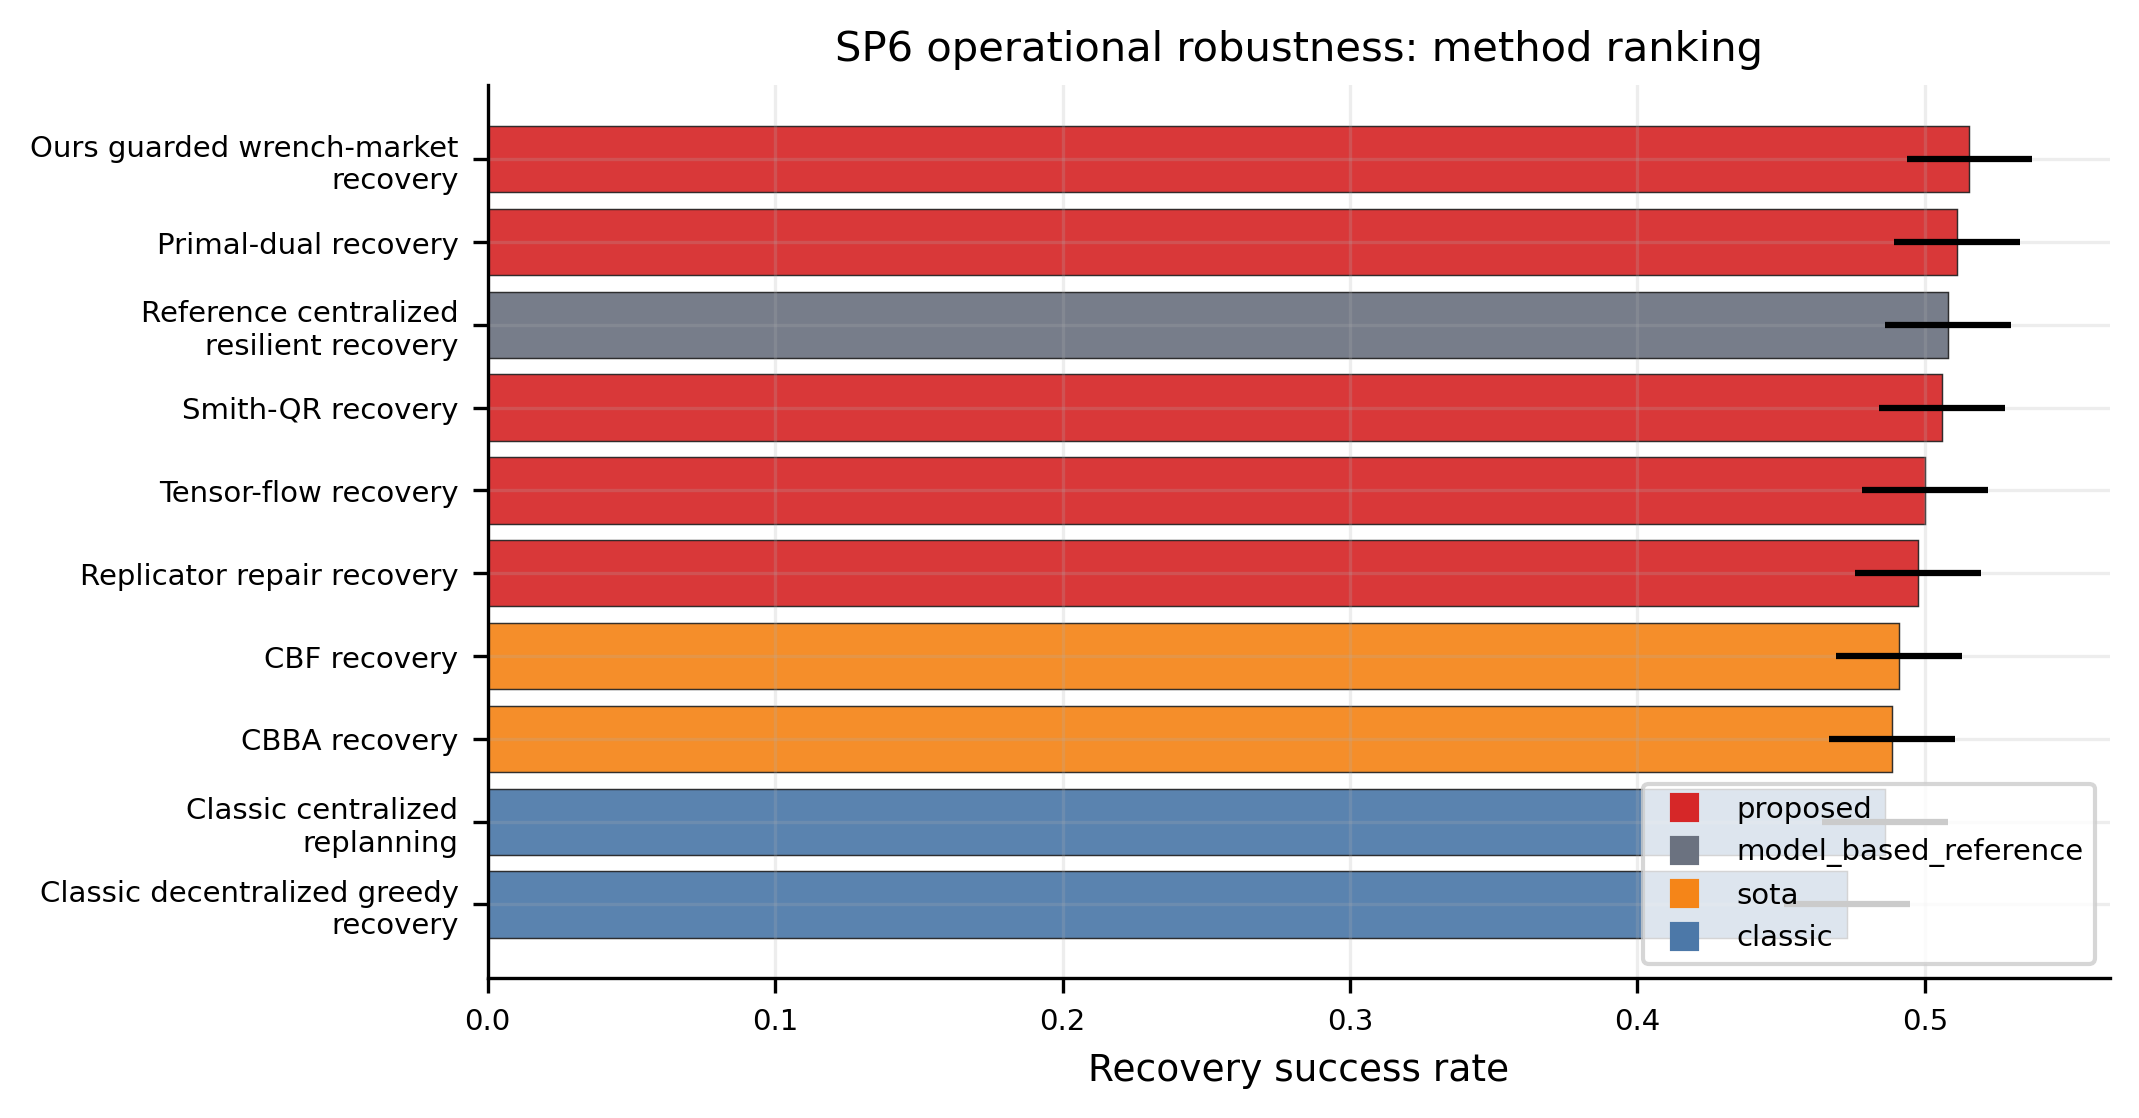
\includegraphics[width=\linewidth]{figures/fig-sp6-primary.png}
\end{minipage}\hfill
\begin{minipage}[t]{0.49\textwidth}
\centering
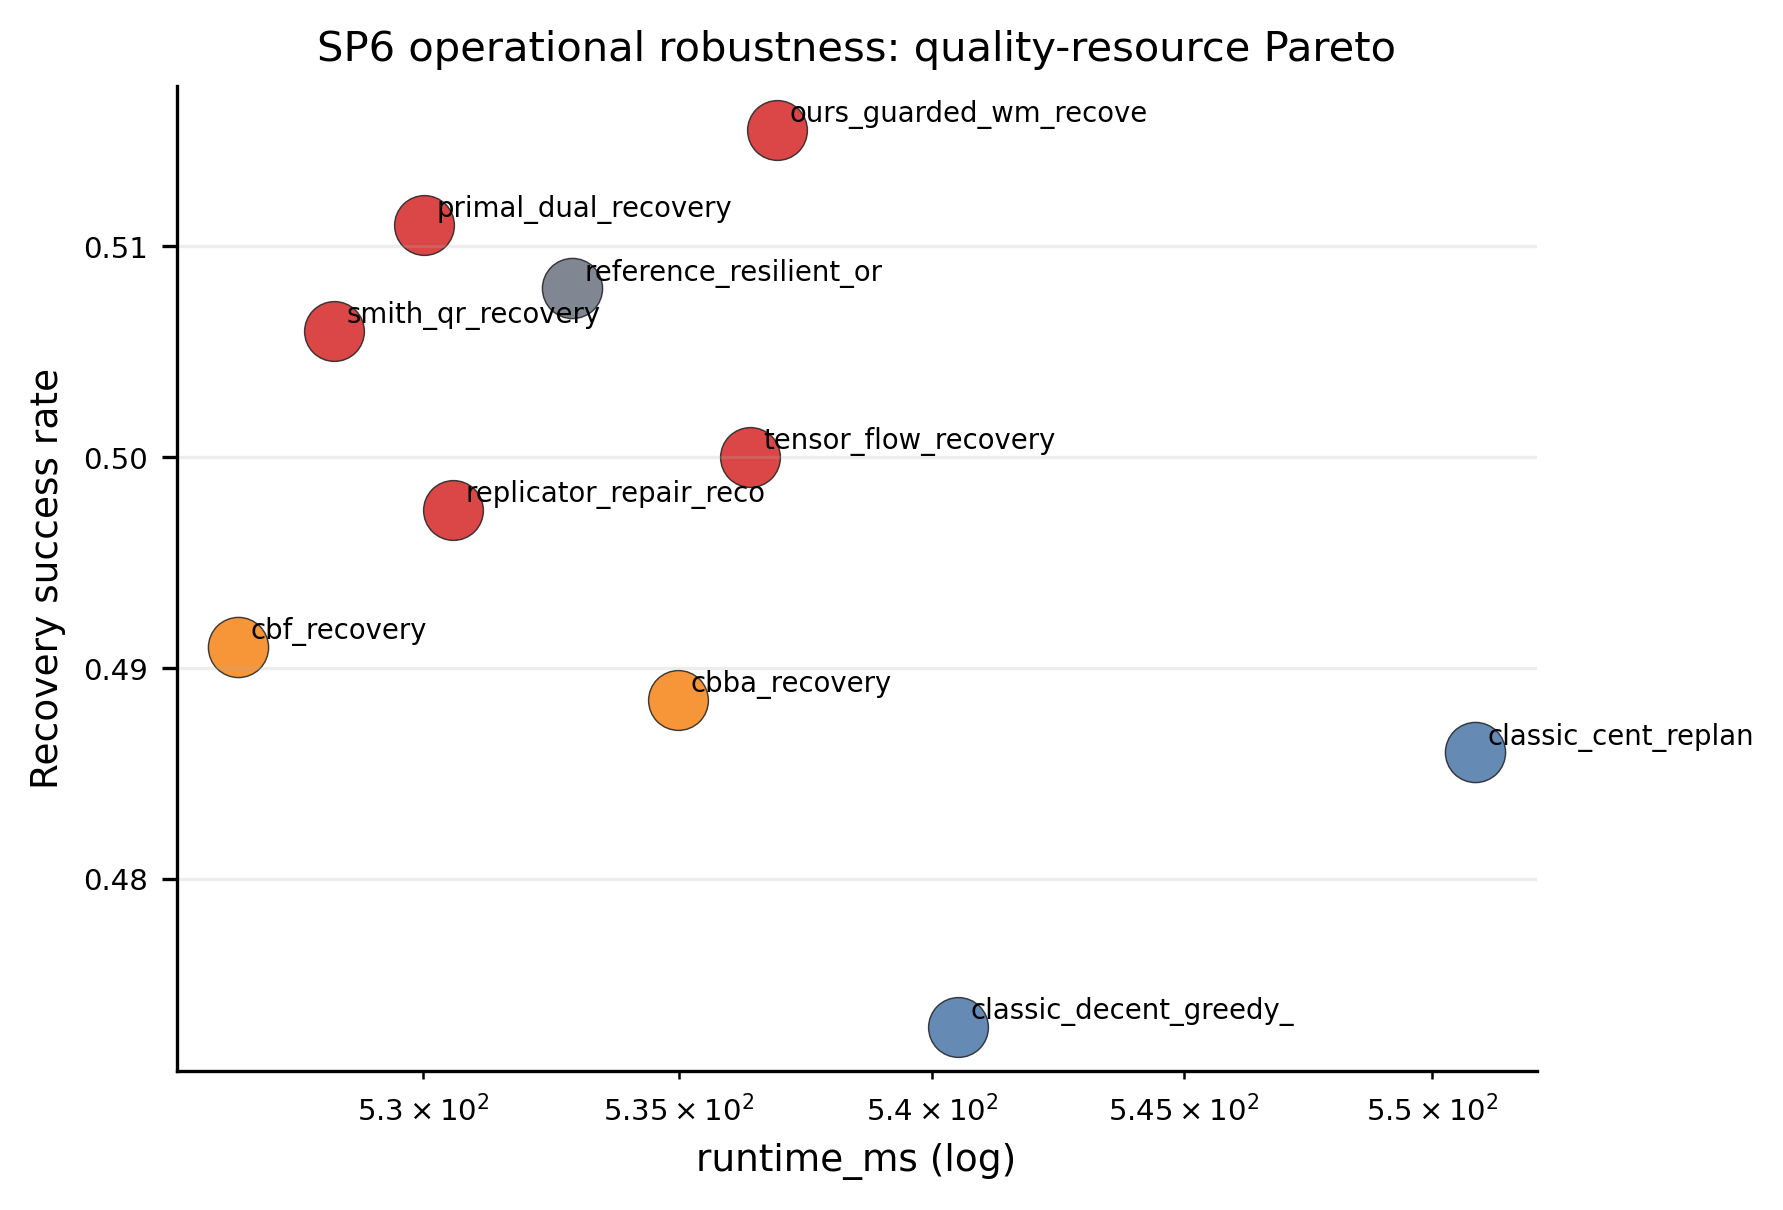
\includegraphics[width=\linewidth]{figures/fig-sp6-pareto.png}
\end{minipage}
\caption[Resultados principales de SP6]{Completitud y relación entre calidad y recursos durante la recuperación.}
\viuownsource
\label{fig:sp6-primary}
\label{fig:sp6-pareto}
\end{figure}

El mercado \emph{wrench} con guardia obtiene $0{,}7117$ de completitud, $0{,}5155$ de recuperación y $0{,}9673$ de factibilidad posterior al evento. Primal-dual alcanza $0{,}7095$ de completitud y la referencia resiliente $0{,}7089$. Smith-QR registra $0{,}7073$. CBBA y \emph{greedy} descienden a $0{,}6958$ y $0{,}6890$. Las tasas de pérdida de carga son $0{,}2883$ para la variante con guardia y $0{,}3110$ para \emph{greedy}.

La reducción de pérdida frente a \emph{greedy} es $-0{,}0227$, con $p_{\rm Holm}<0{,}001$. La brecha frente a CBBA disminuye en $0{,}0658$, también con $p_{\rm Holm}<0{,}001$. La completitud supera a Smith-QR en $0{,}0044$, pero el contraste no respalda una diferencia, $p_{\rm Holm}=0{,}1962$. La comparación global obtiene $W=0{,}0753$. El efecto es consistente y pequeño, acorde con una campaña donde varios métodos reparan la mayoría de los eventos recuperables.

\paragraph{Alcance.} La guardia reduce reparaciones que conservarían una carga inviable. Su ventaja aparece en pérdida y brecha, sin dominio global de completitud. El catálogo de eventos no incluye averías progresivas ni fallos correlacionados de una zona.
